%%%%%%%%%%%%%%%%%%%%%%%%%%%%%%%%%%%%%%%%%
% Beamer Presentation
% LaTeX Template
% Version 1.0 (10/11/12)
%
% This template has been downloaded from:
% http://www.LaTeXTemplates.com
%
% License:
% CC BY-NC-SA 3.0 (http://creativecommons.org/licenses/by-nc-sa/3.0/)
%
%%%%%%%%%%%%%%%%%%%%%%%%%%%%%%%%%%%%%%%%%

%----------------------------------------------------------------------------------------
%	PACKAGES AND THEMES
%----------------------------------------------------------------------------------------

\documentclass{beamer}

\mode<presentation> {

% The Beamer class comes with a number of default slide themes
% which change the colors and layouts of slides. Below this is a list
% of all the themes, uncomment each in turn to see what they look like.

%\usetheme{default}
%\usetheme{AnnArbor}
%\usetheme{Antibes}
%\usetheme{Bergen}
%\usetheme{Berkeley}
%\usetheme{Berlin}
\usetheme{Boadilla}
%\usetheme{CambridgeUS}
%\usetheme{Copenhagen}
%\usetheme{Darmstadt}
%\usetheme{Dresden}
%\usetheme{Frankfurt}
%\usetheme{Goettingen}
%\usetheme{Hannover}
%\usetheme{Ilmenau}
%\usetheme{JuanLesPins}
%\usetheme{Luebeck}
%\usetheme{Madrid}
%\usetheme{Malmoe}
%\usetheme{Marburg}
%\usetheme{Montpellier}
%\usetheme{PaloAlto}
%\usetheme{Pittsburgh}
%\usetheme{Rochester}
%\usetheme{Singapore}
%\usetheme{Szeged}
%\usetheme{Warsaw}

% As well as themes, the Beamer class has a number of color themes
% for any slide theme. Uncomment each of these in turn to see how it
% changes the colors of your current slide theme.

%\usecolortheme{albatross}
%\usecolortheme{beaver}
%\usecolortheme{beetle}
%\usecolortheme{crane}
%\usecolortheme{dolphin}
\usecolortheme{dove}
%\usecolortheme{fly}
%\usecolortheme{lily}
%\usecolortheme{orchid}
%\usecolortheme{rose}
%\usecolortheme{seagull}
%\usecolortheme{seahorse}
%\usecolortheme{whale}
%\usecolortheme{wolverine}

%\setbeamertemplate{footline} % To remove the footer line in all slides uncomment this line
%\setbeamertemplate{footline}[page number] % To replace the footer line in all slides with a simple slide count uncomment this line

%\setbeamertemplate{navigation symbols}{} % To remove the navigation symbols from the bottom of all slides uncomment this line
}
\usepackage{graphicx} % Allows including images
\usepackage{booktabs} % Allows the use of \toprule, \midrule and \bottomrule in tables
\usepackage{ifthen}
\usepackage{uniprpres}
\usepackage{color}
\usepackage{multicol}
\usepackage{pgfplots}
\usepackage{gensymb}
\usepackage[latin1]{inputenc}
\usepackage[italian]{babel}

\setlength{\columnseprule}{1pt}

%----------------------------------------------------------------------------------------
%	TITLE PAGE
%----------------------------------------------------------------------------------------



\titolo{Estrazione di punti operazione per AGV industriali da scansioni laser terrestri}
\titoloIng{Automatic extraction of AGV pickup and delivery points from terrestrial laser scan data}
\laureando{Giorgio Ghisotti}
\annoaccademico{2016-2017}
\corsodilaurea{Ingegneria Informatica, Elettronica e delle Telecomunicazioni}
\relatore[Chiar.mo Prof.]{Jacopo Aleotti}
\correlatorea[Ing.]{Mikhail Giorgini}

\begin{document}
\maketitle

\begin{frame}
	\frametitle{Il Problema}
	\vskip 0.6cm
	\begin{center}
		\begin{huge}
			Individuare punti operazione per carrelli automatici (AGV)
		\end{huge}
	\end{center}
	\vskip 0.2cm
	\begin{center}
		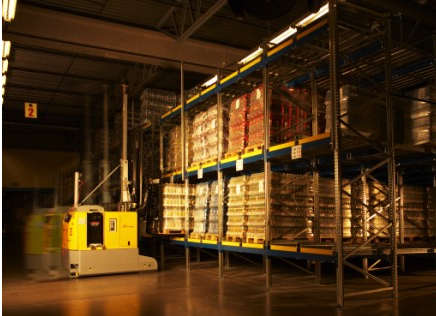
\includegraphics[scale=0.5]{Img/LGV/op}
	\end{center}
\end{frame}

\begin{frame}
	\frametitle{Come si procedeva prima}
	\begin{columns}
		\column{0.6\textwidth}
			\begin{large}
				\begin{itemize}
					\item Misurazioni manuali sul campo
					\begin{itemize}
						\item Effettuate conducendo un carrello in giro per il magazzino
						\item Richiedevano mesi
						\item Rendevano inagibili parti del magazzino durante la procedura
					\end{itemize}
					\item Individuazione manuale con l'aiuto di un programma
					\begin{itemize}
						\item Procedura tediosa
						\item Richiede settimane
						\item Occupa l'operatore per molto tempo
					\end{itemize}
				\end{itemize}
			\end{large}
		\column{0.4\textwidth}
			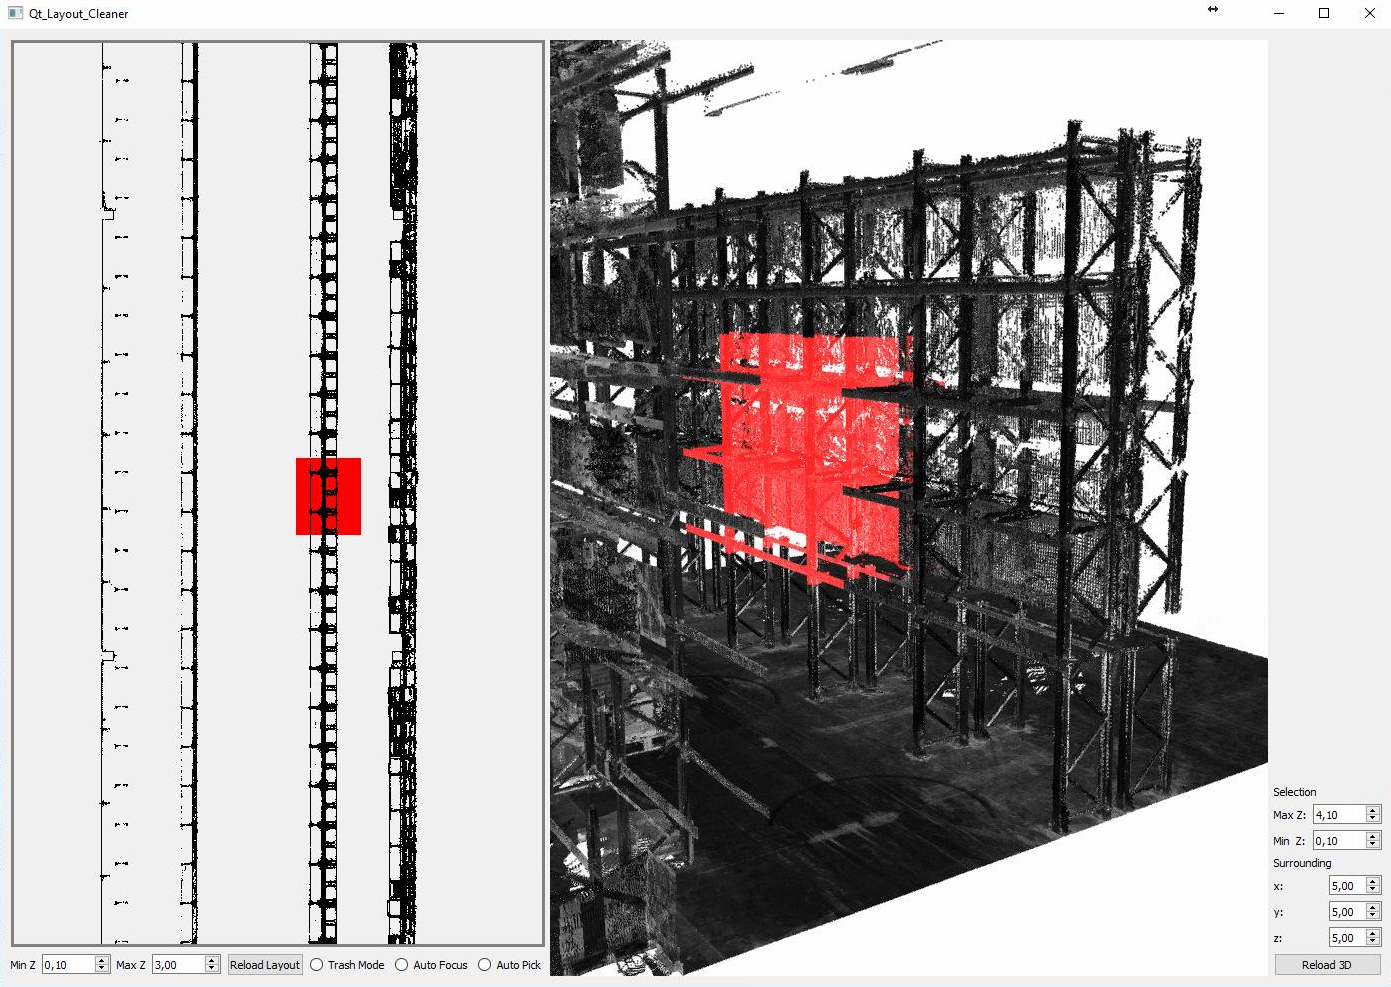
\includegraphics[width=\textwidth]{Img/LGV/select}
	\end{columns}
\end{frame}

\begin{frame}
	\frametitle{Point Cloud}
	\begin{columns}
		\column{0.6\textwidth}
		\begin{itemize}
			\item Si usano delle scansioni laser dei magazzini
			\item Gli strumenti di aquisizione sono sensori laser ad alta precisione
			\item I dati ottenuti sono sotto forma di Point Cloud
			\item Ogni punto ha le sue coordinate in 3D
			\vskip 0.6cm
			\item La Point Cloud di un magazzino contiene \textit{centinaia di miliardi} di punti
		\end{itemize}
		\column{0.4\textwidth}
		\begin{center}
			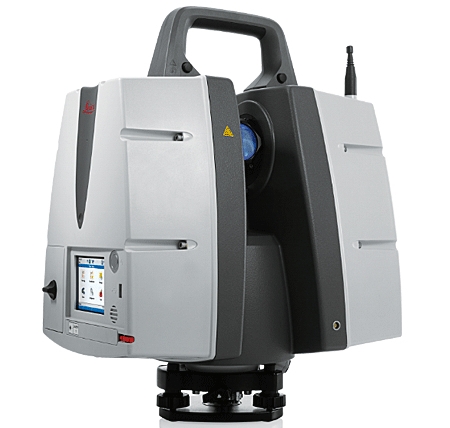
\includegraphics[width=0.6\textwidth]{Img/LGV/Leica_ScanStation_P40}
			\vskip 0.5cm
			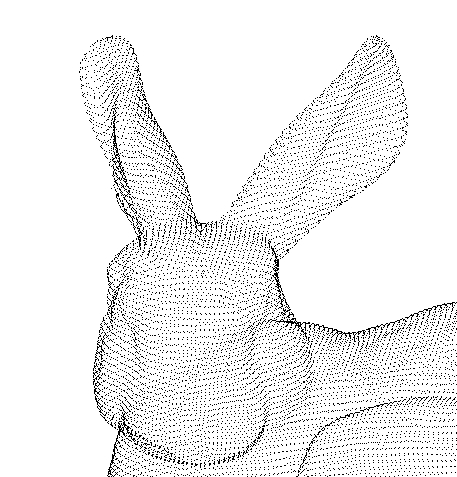
\includegraphics[width=0.6\textwidth]{Img/LGV/bunny_crop}
		\end{center}
	\end{columns}
\end{frame}

\begin{frame}
	\frametitle{Dalla Point Cloud al 2D}
	\begin{columns}
		\column{0.4\textwidth}
			\begin{enumerate}
				\item Si assegna un valore ai punti in base alla curvatura della superficie
				\item Si accumulano i valori generati su una griglia in 2D
				\item Si assegna un colore in scala di grigi alle caselle della griglia in base al colore
			\end{enumerate}
		\column{0.5\textwidth}
			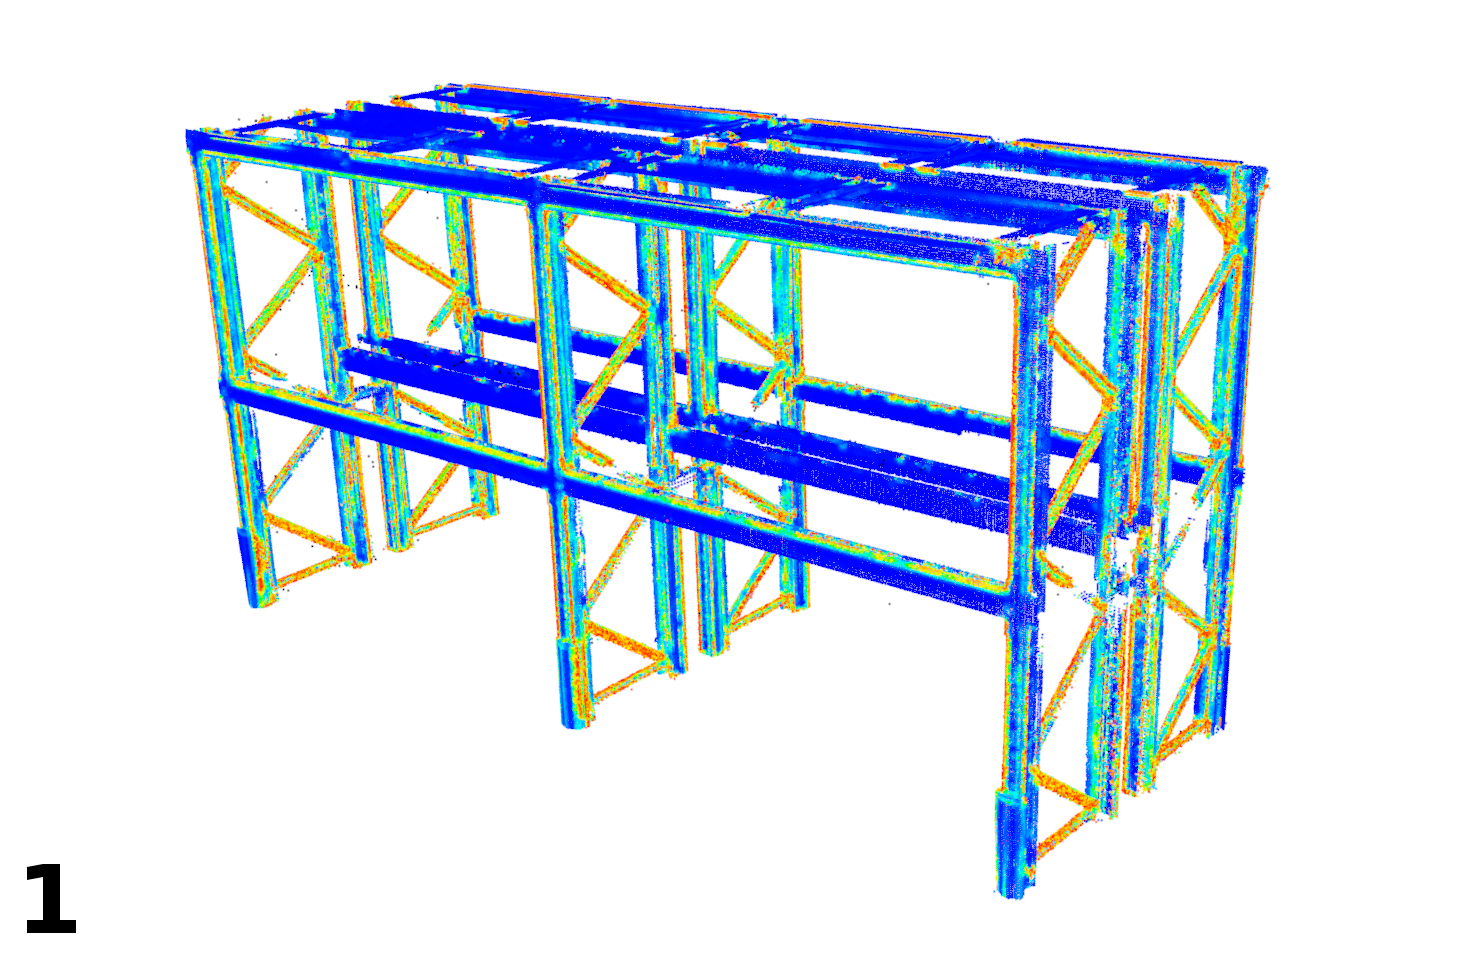
\includegraphics[width=0.6\textwidth]{Img/CURVATURE/CURVATURE_02_num}
			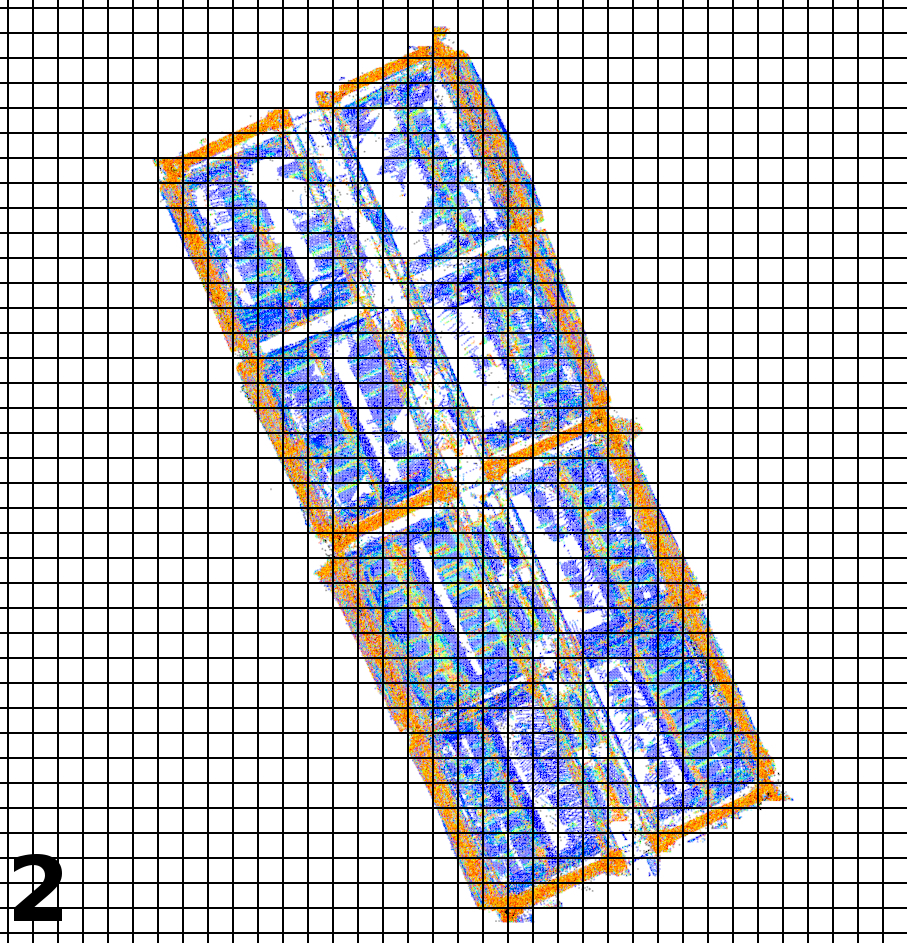
\includegraphics[width=0.4\textwidth]{Img/CURVATURE/CURVATURE_01_grid_num}
			\vskip 0.5cm
			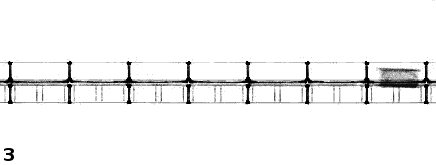
\includegraphics[width=\textwidth]{Img/2D/mag_2d_num_inv}
	\end{columns}
\end{frame}

\begin{frame}
	\frametitle{Individuazione con OpenCV}
	\begin{columns}
		\column{0.5\textwidth}
			\begin{itemize}
				\item La libreria OpenCV permette di riconoscere gli oggetti automaticamente
				\vskip 0.3cm
				\item Basta indicare al sistema un template
				\vskip 0.8cm
				\item Sono necessari alcuni filtri
			\end{itemize}
		\column{0.4\textwidth}
			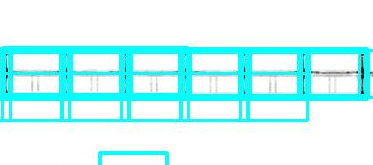
\includegraphics[width=\textwidth]{Img/2D/nofilter_crop_inv}
			\vskip 0.5cm
			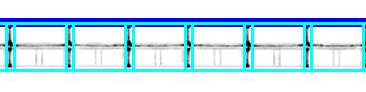
\includegraphics[width=\textwidth]{Img/2D/found_curves_red_crop_inv}
	\end{columns}
\end{frame}

\begin{frame}
	\frametitle{Filtri}
	\begin{multicols}{2}
		\begin{itemize}
			\item Soglia
				\begin{itemize}
					\item Scarta i risultati con valore troppo basso
				\end{itemize}
			\item NMS
				\begin{itemize}
					\item Non Maximum Suppression
					\item Trova i picchi locali
					\item Elimina i risultati troppo vicini ai picchi
				\end{itemize}
			\item Filtro di fila
				\begin{itemize}
					\item Stima le file di rack con RANSAC
					\item Scarta i risultati troppo lontani dalle file
				\end{itemize}
		\end{itemize}
	\columnbreak
			\begin{center}
				{\bfseries Soglia severa\\
				$\Downarrow$\\
				Filtro NMS\\
				$\Downarrow$\\
				Stima delle file con RANSAC\\
				$\Downarrow$\\
				Soglia permissiva\\
				$\Downarrow$\\
				Filtro di fila\\
				$\Downarrow$\\
				Filtro NMS}
			\end{center}
	\end{multicols}
\end{frame}

\begin{frame}
\pgfplotsset{width = \textwidth}
	\frametitle{Risultati}
	\begin{columns}
		\column{0.6\textwidth}
		
		\begin{itemize}
			\item Mediamente il sistema trova quasi tutti gli oggetti cercati
			\item Il sistema genera spesso qualche falso positivo
			\item I falsi positivi sono accettabili in basso numero
			\item Togliere manualmente un punto operazione dal sistema � preferibile ad aggiungerne uno
			\item I tempi di esecuzione del sistema sono di poche ore al massimo
			\item Una volta generata l'immagine del magazzino la ricerca richiede pochi minuti
		\end{itemize}
		
		\column{0.4\textwidth}
		\begin{center}
			\begin{tiny}
				\begin{tikzpicture}
					\begin{axis}[
						ybar,
						enlargelimits=0.15,
						legend style={at={(0.5,-0.2)},
							anchor=north,legend columns=-1},
						ylabel={Falsi positivi/Corretti (\%)},
						symbolic x coords={-20\degree,-10\degree,0\degree,%
							10\degree,20\degree,180\degree},
						xtick=data,
						nodes near coords,
						nodes near coords align={vertical},
						]
						\addplot[draw=gray, fill=gray, bar width=0.06\textwidth] coordinates {
							(-20\degree,8.7) (-10\degree,1.8) (0\degree,1.8)
							(10\degree ,1.3) (20\degree,3.7) (180\degree,2.7)
						};
					\end{axis}
				\end{tikzpicture}
				\begin{tikzpicture}
					\begin{axis}[
						ybar,
						enlargelimits=0.15,
						legend style={at={(0.5,-0.2)},
							anchor=north,legend columns=-1},
						ylabel={Numero medio di falsi positivi},
						symbolic x coords={-20\degree,-10\degree,0\degree,%
							10\degree,20\degree,180\degree},
						xtick=data,
						nodes near coords,
						nodes near coords align={vertical},
						]
						\addplot[draw=gray, fill=gray, bar width=0.06\textwidth] coordinates {
							(-20\degree,2.6) (-10\degree,0.2) (0\degree,0.2)
							(10\degree ,0.5) (20\degree,1.1) (180\degree,1)
						};
					\end{axis}
				\end{tikzpicture}
			\end{tiny}
		\end{center}
	\end{columns}
\end{frame}

\begin{frame}
	\frametitle{Limitazioni}
	\begin{columns}
		\column{0.6\textwidth}
		\begin{itemize}
			\item Il sistema dipende dalla possibilit� di generare immagini adatte
			\item Il filtro NMS pu� generare aberrazioni con template dalla forma particolare
			\item La funzione RANSAC che stima le file di rack potrebbe sbagliare in un magazzino con molte file parallele
			\item Nell'implementazione corrente il sistema non cerca oggetti ruotati rispetto al template
		\end{itemize}
		\column{0.4\textwidth}
		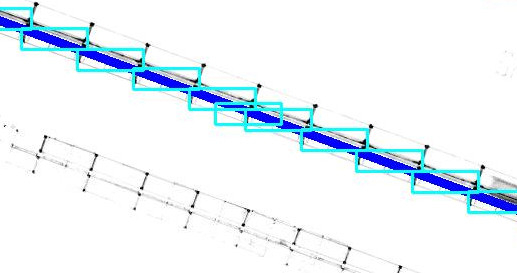
\includegraphics[width=\textwidth]{Img/2D/aberrazioni_crop_inv}\\
		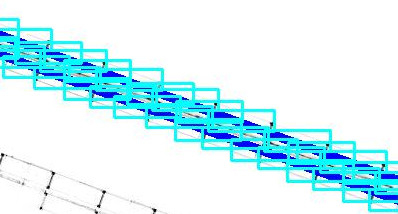
\includegraphics[width=\textwidth]{Img/2D/aberrazioni0_crop_inv}
	\end{columns}
\end{frame}

\begin{frame}
	\frametitle{Sviluppi futuri}
		\begin{center}
			\begin{large}
				\begin{itemize}
					\item Ricerca di corrispondenze ruotate
					\vskip 1cm
					\item Stima di un raggio per NMS adatto al template fornito
					\vskip 1cm
					\item Verifica di correttezza delle file ipotizzate
				\end{itemize}
			\end{large}
		\end{center}
\end{frame}

\begin{frame}
	\frametitle{Grazie}
	\begin{center}
		\vskip 3cm
		\begin{huge}
				Grazie per l'attenzione!
		\end{huge}
		\vskip 3cm
		Giorgio Ghisotti\\
		giorgio.ghisotti@studenti.unipr.it
	\end{center}
\end{frame}


























\end{document} 